\documentclass[11pt,a4paper]{article}

\usepackage[utf8]{inputenc}
\usepackage[T1]{fontenc}
\usepackage{lmodern}
\usepackage[margin=2.4cm]{geometry}
\usepackage{amsmath,amssymb,amsthm,mathtools}
\usepackage{bm}
\usepackage{booktabs,array,float}
\usepackage{enumitem}
\usepackage{microtype}
\usepackage{graphicx}
\usepackage{xcolor}
\usepackage[numbers,sort&compress]{natbib}
\usepackage[colorlinks=true,linkcolor=blue!45!black,citecolor=blue!45!black,urlcolor=blue!45!black]{hyperref}
\usepackage{cleveref}

\newtheoremstyle{thmstyle}{\topsep}{\topsep}{\itshape}{}{\bfseries}{.}{.5em}{}
\theoremstyle{thmstyle}
\newtheorem{theorem}{Theorem}[section]
\newtheorem{lemma}[theorem]{Lemma}
\newtheorem{proposition}[theorem]{Proposition}
\newtheorem{corollary}[theorem]{Corollary}
\theoremstyle{definition}
\newtheorem{definition}[theorem]{Definition}
\newtheorem{axiom}{Axiom}
\newtheorem{example}[theorem]{Example}
\theoremstyle{remark}
\newtheorem{remark}[theorem]{Remark}

\crefname{axiom}{Axiom}{Axioms}
\Crefname{axiom}{Axiom}{Axioms}

\newcommand{\R}{\mathbb{R}}
\newcommand{\N}{\mathbb{N}}
\newcommand{\med}{\mathfrak{M}}
\newcommand{\Gph}{G}
\newcommand{\V}{V}
\newcommand{\E}{E}
\newcommand{\wt}{w}
\newcommand{\cut}{\partial}
\newcommand{\flo}{\beta}
\newcommand{\res}{\rho}
\newcommand{\sep}{\sigma}
\newcommand{\kap}{\kappa}
\newcommand{\comp}{\diamond}
\newcommand{\abs}[1]{\lvert#1\rvert}
\newcommand{\co}{\complement}
\newcommand{\eps}{\varepsilon}

\title{\textbf{A Residual Algebra for Catalytic Composition:\\[2pt]
Derived Floors, the Telescoping Obstruction,\\
and Closure as a Termination Criterion}}

\author{%
Kundai Farai Sachikonye\\
\small Technical University of Munich\\
\small \texttt{kundai.sachikonye@tum.de}}

\date{\today}

\begin{document}
\maketitle

\begin{abstract}
\noindent
We develop an algebra for events that reduce the uncertainty of a bounded
observer about a target, and for the composition of such events into
cascades. The algebra is built on one quantity, the \emph{residual}: the
irreducible remainder of an identification that cannot be completed. We
prove that the residual is strictly positive whenever identification proceeds
by comparison against a whole that no finite stage exhausts, so that the
positive floor central to the algebra is \emph{derived} rather than posited.
On this floor we define the \emph{catalytic power} $\kap$ of an event as the
fraction of the remaining distance to the floor that the event closes, and
prove that catalytic powers compose by the multiplicative law
$\kap(\gamma_1\comp\gamma_2)=1-(1-\kap_1)(1-\kap_2)$, that composition is
associative and commutative with identity, that the floor is never attained
in finitely many steps, and that convergence to the floor under an infinite
cascade holds if and only if $\sum_i\kap_i=\infty$. We then isolate an
obstruction that invalidates the obvious empirical test of the composition
law: when the powers of the constituent events are estimated from the same
state sequence as the cascade outcome, the multiplicative prediction and the
measurement are the \emph{same algebraic expression}, and any correlation
between them is an identity rather than evidence. We prove this
(\emph{Telescoping Theorem}), give the exact condition under which it holds,
and prove that replacing instance-specific powers by type-averaged powers
breaks the identity, so that the resulting test has a genuine null. We
characterise the residual variance decomposition that determines the power of
that test, and show the test is informative precisely when between-type
variance of $\kap$ exceeds within-type variance. Finally we define
\emph{closure}---a termination criterion under which a cascade is complete
when no further available event can carry the observer into a
state-equivalence class not already reached---and prove that closure is
strictly stronger than any fixed threshold on attained uncertainty, that
every cascade over a finite event registry reaches closure in finitely many
steps, and that closure resolves into exactly two outcomes: convergence on a
single class, or a contested outcome whose honest report is a declared
plurality of classes rather than a selected representative. All results are
proved from stated definitions, and all are checked numerically against
constructed instances; the accompanying computations report both the
confirmations and the one regime in which the composition test is shown to
have no power.
\end{abstract}

\noindent\textbf{Keywords:} residual algebra; catalytic composition;
multiplicative law; derived floor; telescoping identity; type-averaged
estimation; closure; termination criteria; bounded observers.

\tableofcontents

% =====================================================================
\section{Introduction}
\label{sec:intro}
% =====================================================================

\subsection{The question}

Consider an observer that reduces its uncertainty about a target by a
sequence of events: an experiment that narrows a hypothesis space, a
measurement that discriminates among candidate states, a physiological
transition that increases the coherence of a system, an inferential step
that rules out alternatives. Each event closes part of a gap. The question
this paper answers is: \emph{how do such events compose?} If one event
closes a known fraction of the gap and a second event closes a known
fraction, what fraction does the pair close, and what law governs the
sequence of many?

The question has an obvious candidate answer and a less obvious correct
one. The obvious answer is that the reductions add. The correct answer, for
any process in which each event acts on the gap that remains after its
predecessors, is that the \emph{residuals} multiply: what survives two
events is what survives the first, further reduced by the second, so the
surviving fractions compose by product and the closed fractions compose by
$1-(1-\kap_1)(1-\kap_2)$. This is not a modelling choice. It follows from
the definition of ``fraction of the remaining gap'' together with the
requirement that the gap be measured from a fixed floor, and we prove it in
\Cref{sec:composition}.

The substance of the paper lies in three places beyond this law. First, the
floor from which the gap is measured cannot be posited without cost: if it
is set to zero the algebra degenerates and the powers are undefined at
convergence; if it is set to an arbitrary positive constant the algebra is
parameter-dependent and its predictions unfalsifiable. We show
(\Cref{sec:floor}) that a strictly positive floor is \emph{forced} by the
structure of identification itself, provided identification proceeds by
comparison against a whole that no finite stage exhausts.

Second, the composition law admits an apparently decisive empirical test
that is in fact vacuous. If the powers of individual events are estimated
from the same sequence of states from which the cascade outcome is measured,
the multiplicative prediction reduces, by cancellation, to the measurement
itself; the two agree exactly and the agreement carries no information. We
state and prove this obstruction (\Cref{sec:telescoping}) because it is easy
to encounter and easy to mistake for a striking confirmation. We then show
what must be changed for the test to have content.

Third, a cascade must know when to stop. The usual criterion---continue
until attained uncertainty falls below a threshold---is provably inadequate,
because a single internally consistent line of evidence can satisfy any
threshold while an unexamined alternative line would have reached an
incompatible conclusion. We define an alternative criterion
(\Cref{sec:closure}), prove it strictly stronger, and prove that it
terminates with exactly two possible verdicts, one of which is an honest
declaration that no single answer is supported.

\subsection{What is assumed}

We assume one structural fact, stated precisely in \Cref{ax:noncomp}: that
identification of a part proceeds by comparison against the rest, and that
the rest is not exhausted at any finite stage. Everything else is derived.
In particular the positive floor, which in many treatments is an axiom, is
here a theorem (\Cref{thm:floor-derived}). We do not assume any probability
measure, any prior, any noise model, or any parametric family. The algebra
is measure-free: its single quantity is a separation cost on a finite
weighted graph, and its single law is a product.

\subsection{Relation to existing work}

The multiplicative structure we derive is formally the survival-function
composition familiar from reliability theory \citep{barlow1975}, and the
geometric convergence it produces is the standard behaviour of a contraction
\citep{banach1922}. What distinguishes the present treatment is that the
contraction factor is not fitted: it is a ratio of separation costs on a
graph whose floor is derived. The residual quantity we use is a minimum cut,
and we rely on the max-flow--min-cut correspondence and Menger's theorem for
its structural properties \citep{menger1927,fordfulkerson1956}. The
information-theoretic reading of untracked residuals in
\Cref{sec:interpretation} uses Shannon entropy in its original sense
\citep{shannon1948,cover2006}. The termination criterion of
\Cref{sec:closure} is related in spirit to the stopping rules of optimal
experimental design \citep{lindley1956,chaloner1995}, but differs
essentially: those rules stop when expected information gain falls below a
threshold, whereas closure stops when the reachable set of \emph{outcomes}
ceases to grow, a condition that is not a function of any gain magnitude.
The distinction between a threshold criterion and an exhaustion criterion is
made precise in \Cref{thm:closure-stronger}. Our insistence on reporting a
contested outcome rather than a selected representative parallels the
literature on conflicting evidence in belief functions
\citep{dempster1967,shafer1976}, though we reach it by a different route and
without a combination rule.

\subsection{Organisation}

\Cref{sec:setting} fixes the setting. \Cref{sec:floor} derives the floor.
\Cref{sec:power} defines catalytic power and establishes its elementary
properties. \Cref{sec:composition} proves the composition law and its
consequences, including the convergence criterion.
\Cref{sec:telescoping} proves the telescoping obstruction and the
type-averaged correction. \Cref{sec:power-analysis} characterises when the
corrected test has statistical power. \Cref{sec:closure} develops closure.
\Cref{sec:interpretation} gives the three readings of a residual.
\Cref{sec:validation} reports numerical verification.
\Cref{sec:scope} states scope and limitations.

% =====================================================================
\section{The setting}
\label{sec:setting}
% =====================================================================

We work with finite weighted graphs throughout. This is not a restriction on
the phenomena modelled but a commitment about the observer: an observer with
finite descriptive resources represents its situation by finitely many
distinctions, and each distinction costs something to draw.

\begin{definition}[Finite weighted graph; cut]
\label{def:graph}
A \emph{finite weighted graph} is a triple $\Gph=(\V,\E,\wt)$ with $\V$
finite, $\E\subseteq\binom{\V}{2}$, and $\wt\colon\E\to(0,\infty)$. For
$U\subseteq\V$ the \emph{cut} of $U$ is
$\cut(U)=\{\{u,v\}\in\E: u\in U,\ v\notin U\}$, and its weight is
$\wt(\cut(U))=\sum_{e\in\cut(U)}\wt(e)$.
\end{definition}

\begin{definition}[Contact graph; medium]
\label{def:contact}
A \emph{contact graph} is a connected finite weighted graph $\Gph$ together
with a distinguished vertex $\med\in\V$, the \emph{medium}, representing
the rest of the whole against which parts are told apart. Vertices other
than $\med$ are \emph{items}. An edge $\{u,v\}$ records that $u$ and $v$
have been separated, and $\wt(\{u,v\})$ is the cost of that separation.
\end{definition}

\begin{remark}[The medium is the rest, not a background]
\label{rem:medium}
The medium is not an environment in which items sit; it is the totality of
what an item is not, considered as a single vertex. Its role is to be the
counterparty of every identification. An item is not individuated against
some items and not others: it is individuated against everything else at
once, and the cost of doing so is the weight of the cheapest cut separating
it from $\med$.
\end{remark}

\begin{definition}[Separation cost; resting cut]
\label{def:sepcost}
For an item $v$, the \emph{separation cost} is
\[
\sep(v)\;=\;\min\{\wt(\cut(U)) : v\in U\subseteq\V\setminus\{\med\}\},
\]
the minimum weight of a cut separating $v$ from the medium. A minimising
$U^{\ast}(v)$ is a \emph{resting side}, and $\cut(U^{\ast}(v))$ the
\emph{resting cut}. The minimum is attained because $\V$ is finite.
\end{definition}

Separation cost is the fundamental observable of the algebra. By the
max-flow--min-cut theorem \citep{fordfulkerson1956} it equals the maximum
flow from $v$ to $\med$, and by Menger's theorem \citep{menger1927} it
counts, in the unweighted case, the maximum number of edge-disjoint paths
that must be severed to disconnect $v$ from the rest. Both readings support
the same intuition: $\sep(v)$ measures how much must be committed to hold
$v$ apart from everything it is not.

\begin{definition}[State; uncertainty]
\label{def:state}
A \emph{state} of an observer with respect to a target is a contact graph
$\Gph$ together with a designated item $v$. The observer's
\emph{uncertainty} in that state is $S:=\sep(v)$, the separation cost of the
target in the observer's current graph. A state with a smaller separation
cost is one in which the target is held apart more cheaply, i.e.\ is better
individuated.
\end{definition}

\begin{remark}[Why cost decreases as knowledge increases]
\label{rem:direction}
It may seem paradoxical that better individuation corresponds to
\emph{lower} cost. The reading is this: an observer that has already drawn
many distinctions in the neighbourhood of $v$ needs to commit little further
to hold $v$ apart, because most of the separating work is already done and
the remaining cheapest cut is small. An observer that has drawn few
distinctions must commit a great deal at once. The quantity $\sep(v)$
therefore measures the \emph{outstanding} commitment, and it is this that
events reduce.
\end{remark}

% =====================================================================
\section{The floor, derived}
\label{sec:floor}
% =====================================================================

The algebra requires a fixed lower bound $\flo$ from which gaps are
measured. We now show this bound need not be assumed.

\begin{definition}[Expanding family; non-completable whole]
\label{def:noncomp}
An \emph{expanding family} is a sequence of contact graphs
$\Gph_0\subseteq\Gph_1\subseteq\Gph_2\subseteq\cdots$, each obtained from
its predecessor by adjoining items and contacts, representing the
progressive elaboration of an observer's distinctions. The whole is
\emph{non-completable} if for every finite stage $k$ there is an item
present in some later stage but absent from $\Gph_k$: no finite stage
exhausts what there is to be told apart.
\end{definition}

\begin{remark}[An order condition, not a cardinality claim]
\label{rem:order}
Non-completability says only that the process of elaboration has no terminal
stage. It does not assert that the whole is a completed infinite set, and no
argument below requires such an assertion. This matters: the results are
about the unavailability of a finishing point to a finite observer, which is
an order-theoretic fact about the family, not a metaphysical one about the
world.
\end{remark}

\begin{axiom}[Identification against a non-completable whole]
\label{ax:noncomp}
Items are identified by comparison against the medium, and the whole is
non-completable in the sense of \Cref{def:noncomp}.
\end{axiom}

\begin{definition}[Identification residual]
\label{def:residual}
To \emph{identify} an item $v$ at stage $k$ is to determine it by comparison
against $\med$ in $\Gph_k$. The identification is \emph{complete} if every
item of the whole has been brought to bear on the comparison. The
\emph{identification residual} $\res(v)$ is the content of the comparison
that remains outstanding; a complete identification has $\res(v)=0$.
\end{definition}

\begin{theorem}[Floor from non-completability]
\label{thm:floor-derived}
Under \Cref{ax:noncomp}, no identification of an item is complete at any
finite stage, and consequently $\res(v)>0$ for every item $v$.
\end{theorem}

\begin{proof}
Suppose $\res(v)=0$ at some finite stage $k$, so the identification of $v$
is complete in $\Gph_k$. By \Cref{def:residual}, completeness requires that
every item of the whole has been brought to bear on the comparison of $v$
against $\med$; every such item is therefore present in $\Gph_k$. Hence
$\Gph_k$ contains the whole, contradicting non-completability
(\Cref{def:noncomp}), which supplies an item absent from $\Gph_k$. Therefore
no finite stage completes the identification and $\res(v)>0$.
\end{proof}

\begin{corollary}[Positive floor]
\label{cor:floor}
There is a constant $\flo>0$ with $\sep(v)\ge\flo$ for every item $v$ of
every stage, and $\wt(e)\ge\flo$ for every contact $e$.
\end{corollary}

\begin{proof}
Put $\flo:=\inf_v\res(v)$ over the items of the family. By
\Cref{thm:floor-derived} each $\res(v)>0$. If $\flo=0$ there are items with
residual arbitrarily close to zero; such an identification is arbitrarily
close to complete, and in the limit completes, which
\Cref{thm:floor-derived} forbids. Hence $\flo>0$. The residual of $v$ is
carried by the contacts of its resting cut, so $\sep(v)\ge\flo$; and each
contact $\{u,v\}$ lies in the cut of the singleton $\{u\}$, whence
$\wt(e)\ge\flo$.
\end{proof}

\begin{corollary}[No sharp identification]
\label{cor:nosharp}
No item is individuated at zero cost, and no state has $S=0$. The attainable
values of the uncertainty $S$ lie in $[\flo,\infty)$.
\end{corollary}

\begin{remark}[Status of the floor]
\label{rem:floor-status}
The floor is not a limitation of an instrument and not a tunable constant.
It is the outstanding remainder of a comparison that cannot be finished, and
its positivity is exactly the statement that the comparison cannot be
finished. Two consequences are used repeatedly below: the denominator
$S-\flo$ appearing in \Cref{def:power} is well defined and positive for
every attainable state above the floor; and the floor is a property of the
observer's situation rather than of any particular event, so it is held
fixed across a cascade.
\end{remark}

\begin{remark}[The floor is estimable, and its positivity is falsifiable]
\label{rem:floor-empirical}
\Cref{thm:floor-derived} predicts an empirical signature. If the floor is
genuine, then estimating $\sep(v)$ as the family expands---as more of the
whole is brought to bear---should exhibit convergence to a strictly positive
asymptote rather than decay toward zero. This is a testable claim and is not
guaranteed by construction.

We stress the contrast with an estimator that defines the floor as the
minimum observed value of $S$ in a finite sample. Such an estimator is
strictly positive whenever the sample is, so it can never return a value
inconsistent with a positivity claim: it has no capacity to falsify. It is
moreover biased upward, a sample minimum being an upper bound on the infimum
of the underlying process, and by \Cref{prop:floor-sensitivity} an
upward-biased floor inflates precisely the powers of the events acting
nearest the floor. The relevant distinction is between \emph{falsification}
and \emph{ordering}: given unboundedly many draws from a process whose
density approaches zero, a sample minimum eventually becomes small and may
then order an unfloored process below a floored one. That ordering is not a
test of positivity, and in the finite-sample regime an experimenter actually
occupies, the sample minimum reports a confidently positive floor for a
process that has none. \Cref{sec:validation} implements both estimators in a
realistic and a large-sample regime and reports the contrast.
\end{remark}

% =====================================================================
\section{Catalytic power}
\label{sec:power}
% =====================================================================

\begin{definition}[Event; catalytic power]
\label{def:power}
An \emph{event} $\gamma$ carries an observer from a state with uncertainty
$S_{\mathrm{before}}>\flo$ to a state with uncertainty $S_{\mathrm{after}}$.
Its \emph{catalytic power} is
\[
\boxed{\ \kap(\gamma)\;=\;\frac{S_{\mathrm{before}}-S_{\mathrm{after}}}
{S_{\mathrm{before}}-\flo}\ }
\]
the fraction of the outstanding gap to the floor that the event closes.
\end{definition}

\begin{definition}[Residual factor]
\label{def:resfactor}
The \emph{residual factor} of an event is $\bar\kap(\gamma):=1-\kap(\gamma)$,
the fraction of the gap that survives it. Explicitly
\[
\bar\kap(\gamma)=\frac{S_{\mathrm{after}}-\flo}{S_{\mathrm{before}}-\flo}.
\]
\end{definition}

The residual factor is the natural coordinate of the algebra: the entire
composition theory is the statement that residual factors multiply, and
every result below is more transparent in $\bar\kap$ than in $\kap$.

\begin{proposition}[Elementary properties]
\label{prop:elementary}
Let $\gamma$ be an event acting on a state with $S_{\mathrm{before}}>\flo$.
Then:
\begin{enumerate}[label=\textup{(\roman*)},leftmargin=2.2em]
\item $\kap(\gamma)\le1$, with equality iff $S_{\mathrm{after}}=\flo$;
\item $\kap(\gamma)>0$ iff the event strictly reduces uncertainty, and
$\kap(\gamma)<0$ iff it strictly increases it;
\item $\kap(\gamma)=0$ iff the event leaves uncertainty unchanged;
\item $\bar\kap(\gamma)\ge0$ for every event whose post-state is attainable,
by \Cref{cor:nosharp}.
\end{enumerate}
\end{proposition}

\begin{proof}
All four are immediate from \Cref{def:power,def:resfactor} and the
positivity of the denominator $S_{\mathrm{before}}-\flo$. For (i), $\kap\le1$
is equivalent to $S_{\mathrm{after}}\ge\flo$, which is
\Cref{cor:nosharp}; equality holds exactly when $S_{\mathrm{after}}=\flo$.
For (iv), $\bar\kap=(S_{\mathrm{after}}-\flo)/(S_{\mathrm{before}}-\flo)\ge0$
since both numerator and denominator are nonnegative, the numerator by
\Cref{cor:nosharp}.
\end{proof}

\begin{remark}[Negative powers are admissible and meaningful]
\label{rem:negative}
Nothing forces $\kap\ge0$. An event that increases the outstanding
commitment---one that draws a distinction which makes the target harder to
hold apart, or that introduces confusable alternatives---has $\kap<0$ and
residual factor exceeding one. The algebra accommodates such events without
modification, and \Cref{sec:validation} exhibits data in which they occur
systematically: transitions away from a dominant attractor state carry large
negative power. Excluding them would amount to assuming that every event is
informative, which is exactly what an experimental apparatus should not
assume.
\end{remark}

\begin{proposition}[Scale invariance]
\label{prop:scale}
Catalytic power is invariant under affine reparametrisation of the
uncertainty that fixes the floor: for $a>0$ and $S\mapsto a(S-\flo)+\flo$,
every $\kap(\gamma)$ is unchanged.
\end{proposition}

\begin{proof}
Both numerator and denominator of \Cref{def:power} scale by $a$:
$\bigl(a(S_{\mathrm{b}}-\flo)-a(S_{\mathrm{a}}-\flo)\bigr)/
\bigl(a(S_{\mathrm{b}}-\flo)\bigr)=
(S_{\mathrm{b}}-S_{\mathrm{a}})/(S_{\mathrm{b}}-\flo)$.
\end{proof}

\Cref{prop:scale} is what makes the algebra portable across substrates. The
units of $S$ are arbitrary; only the position of a state relative to the
floor matters. It also identifies precisely the one quantity that must be
determined per observer before any power can be computed---the floor---and
explains why an error in the floor is not a change of units but a distortion
of every power in the cascade. We return to this sensitivity in
\Cref{prop:floor-sensitivity}.

% =====================================================================
\section{Composition}
\label{sec:composition}
% =====================================================================

\begin{definition}[Cascade]
\label{def:cascade}
A \emph{cascade} is a finite sequence $\gamma_1,\dots,\gamma_n$ of events
applied in order to an observer with fixed floor $\flo$, with the post-state
of $\gamma_i$ the pre-state of $\gamma_{i+1}$. Writing $S_1$ for the initial
and $S_{n+1}$ for the terminal uncertainty, the \emph{net power} of the
cascade is
$\kap_{\mathrm{net}}=(S_1-S_{n+1})/(S_1-\flo)$, i.e.\ the power of the
cascade regarded as a single event.
\end{definition}

\begin{theorem}[Multiplicative composition]
\label{thm:composition}
For any cascade $\gamma_1,\dots,\gamma_n$ over a fixed floor,
\[
\boxed{\ \kap_{\mathrm{net}}
=1-\prod_{i=1}^{n}\bigl(1-\kap(\gamma_i)\bigr)\ }
\]
equivalently, the residual factors multiply:
$\bar\kap_{\mathrm{net}}=\prod_{i=1}^{n}\bar\kap(\gamma_i)$.
\end{theorem}

\begin{proof}
Write $g_i:=S_i-\flo$ for the gap before event $\gamma_i$, so $g_i>0$ for
$i\le n$ by hypothesis and $g_{n+1}\ge0$ by \Cref{cor:nosharp}. By
\Cref{def:resfactor}, $\bar\kap(\gamma_i)=g_{i+1}/g_i$. Hence
\[
\prod_{i=1}^{n}\bar\kap(\gamma_i)
=\prod_{i=1}^{n}\frac{g_{i+1}}{g_i}
=\frac{g_{n+1}}{g_1}
=\frac{S_{n+1}-\flo}{S_1-\flo}
=1-\kap_{\mathrm{net}},
\]
the last equality by \Cref{def:cascade}. Rearranging gives the displayed
formula.
\end{proof}

\begin{remark}[What the law says, and what it does not]
\label{rem:law-content}
\Cref{thm:composition} is a consequence of the definition of catalytic power
as a fraction of an outstanding gap measured from a fixed floor. It is
therefore not, by itself, an empirical claim: given the definitions, it
cannot fail. What \emph{is} empirical is whether a proposed decomposition of
a process into events, with powers estimated independently of the outcome
being predicted, obeys it. This distinction is the entire subject of
\Cref{sec:telescoping}, and neglecting it is the error that section exists
to forestall.
\end{remark}

\begin{corollary}[Algebraic structure]
\label{cor:structure}
Composition $\comp$ defined by
$\kap_1\comp\kap_2:=1-(1-\kap_1)(1-\kap_2)$ makes $(-\infty,1]$ a
commutative monoid with identity $0$ and absorbing element $1$. It is
associative and commutative, and $\kap\comp0=\kap$, $\kap\comp1=1$.
\end{corollary}

\begin{proof}
The map $\kap\mapsto1-\kap$ is a bijection $(-\infty,1]\to[0,\infty)$
carrying $\comp$ to ordinary multiplication, which is associative and
commutative with identity $1$ and absorbing element $0$. Transporting back,
$\comp$ is associative and commutative with identity $0$ and absorbing
element $1$.
\end{proof}

\begin{remark}[Order independence and its limits]
\label{rem:order-indep}
Commutativity in \Cref{cor:structure} is a statement about the composition
of \emph{given} powers, not a claim that events may be reordered in
practice. Reordering a physical cascade may change the powers themselves,
since $\kap(\gamma)$ is defined relative to the state on which $\gamma$
acts. What the corollary says is that if the powers are what they are, the
net effect does not depend on the order in which they are multiplied. The
empirical content of order-independence---that the same event has the same
power wherever it occurs in a cascade---is a separate hypothesis, and is
exactly what the type-averaged test of \Cref{sec:telescoping} probes.
\end{remark}

\begin{proposition}[Diminishing returns]
\label{prop:diminishing}
For a cascade of events with powers $\kap_i\in(0,1)$, the net power is
strictly increasing in each $\kap_i$ and satisfies
$\kap_{\mathrm{net}}<1$ for every finite $n$. The marginal contribution of
$\gamma_{n+1}$ to the net power is
$\kap_{n+1}\prod_{i\le n}(1-\kap_i)$, which decreases geometrically in $n$
whenever the powers are bounded below by a positive constant.
\end{proposition}

\begin{proof}
Monotonicity is clear from
$\partial\kap_{\mathrm{net}}/\partial\kap_j=\prod_{i\ne j}(1-\kap_i)>0$.
Since each $1-\kap_i>0$, the product is positive and $\kap_{\mathrm{net}}<1$.
For the marginal contribution, compose the first $n$ events into
$\kap_{\mathrm{net}}^{(n)}$; then
$\kap_{\mathrm{net}}^{(n+1)}-\kap_{\mathrm{net}}^{(n)}
=(1-\kap_{\mathrm{net}}^{(n)})\kap_{n+1}
=\kap_{n+1}\prod_{i\le n}(1-\kap_i)$. If $\kap_i\ge c>0$ then this is at
most $(1-c)^{n}$, which decays geometrically.
\end{proof}

\begin{corollary}[The floor is not attained in finite time]
\label{cor:not-attained}
No finite cascade of events with powers $\kap_i<1$ brings the uncertainty to
the floor. The gap after $n$ events is $g_1\prod_{i\le n}(1-\kap_i)>0$.
\end{corollary}

\begin{theorem}[Convergence criterion]
\label{thm:convergence}
Let $\gamma_1,\gamma_2,\dots$ be an infinite cascade with powers
$\kap_i\in[0,1)$. Then the uncertainty converges to the floor,
$S_n\to\flo$, if and only if
\[
\sum_{i=1}^{\infty}\kap_i=\infty .
\]
\end{theorem}

\begin{proof}
The gap after $n$ events is $g_{n+1}=g_1\prod_{i\le n}(1-\kap_i)$, so
$S_n\to\flo$ iff $\prod_{i=1}^{\infty}(1-\kap_i)=0$. For $\kap_i\in[0,1)$
take logarithms: $\prod(1-\kap_i)=0$ iff
$\sum_i-\log(1-\kap_i)=\infty$. Since $-\log(1-x)\ge x$ for $x\in[0,1)$, the
divergence of $\sum\kap_i$ implies divergence of the log-sum. Conversely if
$\sum\kap_i<\infty$ then $\kap_i\to0$, and for $x\in[0,\tfrac12]$ one has
$-\log(1-x)\le2x$, so the log-sum is bounded by a constant plus
$2\sum\kap_i<\infty$, whence the product is strictly positive. Thus
$\prod(1-\kap_i)=0$ iff $\sum\kap_i=\infty$.
\end{proof}

\begin{remark}[Interpretation of the criterion]
\label{rem:borel}
\Cref{thm:convergence} has the form of a Borel--Cantelli dichotomy: what
matters is not the size of any individual power but whether the powers are
summable. A cascade of events each closing a rapidly shrinking fraction of
the gap---say $\kap_i=2^{-i}$---never reaches the floor even in the limit,
while a cascade of arbitrarily weak but non-summable events---$\kap_i=1/i$
---does. This distinguishes processes that stall from processes that
converge, using only the sequence of powers.
\end{remark}

\begin{proposition}[Sensitivity to the floor]
\label{prop:floor-sensitivity}
Let the true floor be $\flo$ and let an analysis use $\flo'=\flo+\eps$ with
$\eps$ small relative to the gap. Then the power computed for an event with
true power $\kap$ is
\[
\kap'=\kap\cdot\frac{S_{\mathrm{b}}-\flo}{S_{\mathrm{b}}-\flo-\eps}
=\kap\Bigl(1+\frac{\eps}{S_{\mathrm{b}}-\flo}\Bigr)+O(\eps^2),
\]
so the relative error in $\kap$ is $\eps/(S_{\mathrm{b}}-\flo)$ to first
order. Misestimation of the floor inflates powers of events acting near the
floor and leaves powers of events acting far from it nearly unchanged.
\end{proposition}

\begin{proof}
Substituting $\flo'$ into \Cref{def:power} leaves the numerator
$S_{\mathrm{b}}-S_{\mathrm{a}}$ unchanged and replaces the denominator by
$S_{\mathrm{b}}-\flo-\eps$. The stated ratio and its expansion follow.
\end{proof}

\Cref{prop:floor-sensitivity} is the practical reason
\Cref{rem:floor-empirical} matters. An analysis that sets the floor to the
sample minimum systematically overestimates it---the sample minimum is an
upper bound on the true infimum---and therefore systematically inflates the
powers of exactly those events that operate closest to the floor, which are
the events of greatest interest.

% =====================================================================
\section{The telescoping obstruction}
\label{sec:telescoping}
% =====================================================================

We now isolate the central methodological result of the paper. The
composition law suggests an immediate test: decompose an observed process
into events, compute each event's power, form the multiplicative prediction,
and compare it against the directly measured net power of the cascade. We
show that under the most natural implementation this comparison is an
identity.

\begin{definition}[Instance-specific estimation]
\label{def:instance}
Powers are estimated \emph{instance-specifically} when, for each cascade,
each $\kap(\gamma_i)$ is computed from \Cref{def:power} using the same
observed uncertainties $S_i,S_{i+1}$ that determine the cascade's own
measured net power.
\end{definition}

\begin{theorem}[Telescoping obstruction]
\label{thm:telescoping}
Under instance-specific estimation, the multiplicative prediction and the
measured net power are equal for every cascade, identically:
\[
1-\prod_{i=1}^{n}\bigl(1-\kap(\gamma_i)\bigr)
\;=\;\frac{S_1-S_{n+1}}{S_1-\flo}
\;=\;\kap_{\mathrm{measured}} .
\]
Consequently any goodness-of-fit statistic comparing the two---a Pearson
correlation, a root-mean-square error, a regression slope---takes its
degenerate value ($r=1$, $\mathrm{RMSE}=0$, slope $1$) on every data set
whatsoever, independently of the process generating the data.
\end{theorem}

\begin{proof}
This is \Cref{thm:composition} read as an identity rather than a prediction.
With $g_i=S_i-\flo$, instance-specific estimation gives
$1-\kap(\gamma_i)=g_{i+1}/g_i$ exactly, so the product telescopes:
\[
\prod_{i=1}^{n}\frac{g_{i+1}}{g_i}=\frac{g_{n+1}}{g_1},
\]
whence $1-\prod_i(1-\kap_i)=1-g_{n+1}/g_1=(S_1-S_{n+1})/(S_1-\flo)$, which
is the measured net power. The two quantities are the same function of the
data, so their difference vanishes pointwise and every discrepancy statistic
attains its degenerate value.
\end{proof}

\begin{corollary}[The degenerate test has no null]
\label{cor:no-null}
There is no data set, and no generating process, under which the
instance-specific test fails. It therefore has no power against any
alternative, and a reported agreement carries no evidential weight.
\end{corollary}

\begin{proof}
By \Cref{thm:telescoping} the agreement holds identically, in particular for
data generated by any process whatsoever, including processes violating
every substantive claim of the algebra. A test that cannot fail cannot
discriminate.
\end{proof}

\begin{remark}[Why this is easy to miss]
\label{rem:easy-to-miss}
The obstruction is invisible at the level of the code that implements the
test: the two quantities are computed by different routines, one looping
over constituent events and multiplying, the other differencing the
endpoints of the cascade, and they agree to machine precision. The agreement
looks like a striking confirmation of the composition law across thousands
of cascades. It is instead a restatement of \Cref{thm:composition}. We
record this explicitly because an $r$ of exactly $1.000$ is precisely the
outcome that should prompt suspicion rather than satisfaction, and because
the same structure will arise in any framework whose composition law is a
telescoping product.
\end{remark}

\subsection{The corrected test}

The obstruction arises because the constituent powers and the cascade
outcome are functions of the same numbers. Breaking the identity requires
estimating powers from a source independent of the particular cascade being
predicted. The natural such source is the \emph{type} of an event.

\begin{definition}[Event type; type-averaged power]
\label{def:type}
Let each event carry a \emph{type} $t(\gamma)$ drawn from a finite label
set---for instance the ordered pair of state labels it connects. For a
corpus of observed events, the \emph{type-averaged power} of type $\theta$
is
\[
\bar\kap_\theta=\frac{1}{\abs{\mathcal{T}_\theta}}
\sum_{\gamma\in\mathcal{T}_\theta}\kap(\gamma),
\qquad
\mathcal{T}_\theta=\{\gamma : t(\gamma)=\theta\}.
\]
The \emph{type-averaged prediction} for a cascade
$\gamma_1,\dots,\gamma_n$ is
$\hat\kap=1-\prod_{i=1}^{n}(1-\bar\kap_{t(\gamma_i)})$.
\end{definition}

\begin{theorem}[The type-averaged test is non-degenerate]
\label{thm:nondegenerate}
Suppose some type $\theta$ has at least two instances with distinct powers.
Then there exist cascades for which
$\hat\kap\ne\kap_{\mathrm{measured}}$, and the map from data to the
discrepancy $\hat\kap-\kap_{\mathrm{measured}}$ is not identically zero.
Hence the type-averaged test has a genuine null hypothesis and can fail.
\end{theorem}

\begin{proof}
Let $\theta$ have instances with powers $\kap\ne\kap'$, so
$\bar\kap_\theta$ differs from at least one of them; without loss
$\bar\kap_\theta\ne\kap$. Consider a cascade of length one consisting of
that instance. Then $\kap_{\mathrm{measured}}=\kap$ while
$\hat\kap=\bar\kap_\theta\ne\kap$, so the discrepancy is nonzero. Since the
discrepancy is nonzero on this instance, it is not identically zero as a
function of the data, and the equality $\hat\kap=\kap_{\mathrm{measured}}$
is a substantive restriction rather than an identity.
\end{proof}

\begin{remark}[What the corrected test asks]
\label{rem:what-asks}
The type-averaged test asks a genuine question: \emph{is the catalytic power
a property of the event type, stable across instances, such that composing
type-level powers predicts instance-level outcomes?} A positive answer
supports both the composition law and the claim that the chosen typing
carves the process at its joints. A negative answer is informative in two
distinguishable ways: the typing may be wrong---events of the same nominal
type may not share a power---or the decomposition into events may be wrong.
\Cref{sec:power-analysis} shows how to tell these apart.
\end{remark}

\begin{proposition}[Exact bias of the type-averaged prediction]
\label{prop:bias}
Write $\kap_i=\bar\kap_{t(i)}+\delta_i$, where $\delta_i$ is the deviation
of instance $i$ from its type mean. Then
\[
\frac{1-\kap_{\mathrm{measured}}}{1-\hat\kap}
=\prod_{i=1}^{n}\Bigl(1-\frac{\delta_i}{1-\bar\kap_{t(i)}}\Bigr),
\]
so the prediction is exact if and only if the deviations vanish, and to
first order in small $\delta$,
\[
\hat\kap-\kap_{\mathrm{measured}}
\approx(1-\hat\kap)\sum_{i=1}^{n}\frac{\delta_i}{1-\bar\kap_{t(i)}} .
\]
\end{proposition}

\begin{proof}
By \Cref{thm:composition},
$1-\kap_{\mathrm{measured}}=\prod_i(1-\kap_i)
=\prod_i(1-\bar\kap_{t(i)}-\delta_i)
=\prod_i(1-\bar\kap_{t(i)})\prod_i\bigl(1-\delta_i/(1-\bar\kap_{t(i)})\bigr)$,
and $\prod_i(1-\bar\kap_{t(i)})=1-\hat\kap$ by \Cref{def:type}. Dividing
gives the stated ratio. Expanding the product to first order in $\delta$
yields $1-\sum_i\delta_i/(1-\bar\kap_{t(i)})$, and substituting gives the
approximation.
\end{proof}

\Cref{prop:bias} makes precise what the corrected test measures: the
discrepancy is driven by the within-type deviations $\delta_i$, amplified by
$1/(1-\bar\kap)$ for high-power types. It also shows the deviations enter
additively at leading order, so that cascades whose deviations cancel will
be predicted well even when individual events are poorly typed---a source of
optimism to be guarded against by examining cascade length.

% =====================================================================
\section{When the corrected test has power}
\label{sec:power-analysis}
% =====================================================================

A non-degenerate test may still be uninformative if the data cannot
distinguish its hypotheses. We characterise the regime in which the
type-averaged test discriminates.

\begin{definition}[Variance decomposition]
\label{def:variance}
For a corpus of events with types, let $\mathrm{Var}_{\mathrm{within}}$
denote the mean over types of the variance of $\kap$ within a type, and
$\mathrm{Var}_{\mathrm{between}}$ the variance across types of the type
means $\bar\kap_\theta$. The \emph{type separation ratio} is
\[
\eta=\frac{\mathrm{Var}_{\mathrm{between}}}
{\mathrm{Var}_{\mathrm{between}}+\mathrm{Var}_{\mathrm{within}}}\in[0,1].
\]
\end{definition}

\begin{proposition}[Degeneracy at vanishing separation]
\label{prop:degeneracy}
If $\eta=0$---all type means coincide---then the type-averaged prediction is
the same constant for every cascade of a given length, its correlation with
the measured net power is undefined \textup{(}zero variance in the
predictor\textup{)}, and the test cannot distinguish the multiplicative law
from any competitor that is also a function of the type means alone.
\end{proposition}

\begin{proof}
If all $\bar\kap_\theta$ are equal to a common $\bar\kap$, then
$\hat\kap=1-(1-\bar\kap)^{n}$ depends only on the cascade length $n$. Among
cascades of fixed length the predictor is constant, so its sample variance
is zero and the Pearson correlation is undefined. Any alternative law
computed from the same type means is likewise constant at fixed length,
hence indistinguishable.
\end{proof}

\begin{remark}[The observable that fails]
\label{rem:compression}
\Cref{prop:degeneracy} identifies the failure mode to check before
interpreting any negative result. If the chosen observable maps every state
label into a narrow band---so that all types have nearly equal mean
power---then $\eta\approx0$ and the test is underpowered by construction,
regardless of whether the composition law holds. A negative result in this
regime is evidence about the observable, not about the law.
\Cref{sec:validation} exhibits exactly this situation in one of the three
constructed regimes, and we report it as an absence of power rather than as
a disconfirmation.
\end{remark}

\begin{proposition}[Competing composition laws]
\label{prop:competitors}
The following are distinct functions of the constituent powers and coincide
only in degenerate cases: the multiplicative law
$1-\prod_i(1-\kap_i)$; the additive law $\min(\sum_i\kap_i,1)$; the
geometric-mean law $1-\bigl(\prod_i(1-\kap_i)\bigr)^{1/n}$; and the maximum
law $\max_i\kap_i$. For $n\ge2$ and powers in $(0,1)$ they satisfy
\[
\max_i\kap_i\;\le\;1-\prod_i(1-\kap_i)\;\le\;\min\Bigl(\sum_i\kap_i,1\Bigr),
\]
with both inequalities strict unless some $\kap_i=0$; and the
geometric-mean law is strictly below the multiplicative law for $n\ge2$
whenever $\prod_i(1-\kap_i)<1$.
\end{proposition}

\begin{proof}
For the left inequality, $\prod_i(1-\kap_i)\le1-\max_i\kap_i$ since every
factor is at most $1$ and one factor equals $1-\max_i\kap_i$; negating gives
the claim, with equality iff all other factors are $1$, i.e.\ all other
powers vanish. For the right, expanding $\prod_i(1-\kap_i)\ge1-\sum_i\kap_i$
(Weierstrass) gives $1-\prod_i(1-\kap_i)\le\sum_i\kap_i$, with equality iff
all cross terms vanish, i.e.\ at most one power is nonzero; combining with
$\kap_{\mathrm{net}}\le1$ gives the stated bound. For the geometric mean,
with $P=\prod_i(1-\kap_i)<1$ we have $P^{1/n}>P$ for $n\ge2$, so
$1-P^{1/n}<1-P$.
\end{proof}

\Cref{prop:competitors} supplies the comparison set for the empirical test:
the four laws are ordered and distinct, so a corpus with adequate type
separation can in principle select among them. It also shows that the
multiplicative law is intermediate, which matters for interpretation---a
finding that it outperforms both the additive and the maximum law is a
two-sided result, not a one-sided one.

% =====================================================================
\section{Closure}
\label{sec:closure}
% =====================================================================

A cascade must terminate. The default criterion---stop when the attained
uncertainty falls below a threshold---is inadequate for a reason we can now
make precise.

\begin{definition}[Event registry; reachable set]
\label{def:registry}
An \emph{event registry} $\Gamma$ is a finite set of events available to an
observer. Fixing an initial state, let $\mathcal{C}(\Gamma')$ denote the set
of terminal states reachable by cascades drawn from an invoked subset
$\Gamma'\subseteq\Gamma$, partitioned into equivalence classes under a
specified indistinguishability relation on terminal states.
\end{definition}

\begin{definition}[Closure]
\label{def:closure}
A cascade is \emph{closed} at stage $\Gamma'$ if for every event
$\gamma\in\Gamma\setminus\Gamma'$ not yet invoked, adjoining $\gamma$ adds
no new equivalence class: every terminal state reachable using $\gamma$ lies
in a class already present in $\mathcal{C}(\Gamma')$.
\end{definition}

\begin{theorem}[Closure is strictly stronger than a threshold]
\label{thm:closure-stronger}
For every threshold $\theta$ on attained uncertainty there exist registries
and initial states such that a cascade attains uncertainty below $\theta$
while failing to be closed: an uninvoked event leads to a terminal state in
a distinct equivalence class. Conversely, closure does not entail any
particular attained uncertainty. The two criteria are therefore not ordered
by implication in the direction threshold~$\Rightarrow$~closure, and closure
is the stronger requirement in the sense that it can fail when the threshold
is met.
\end{theorem}

\begin{proof}
Construct a registry with two events $\gamma_A,\gamma_B$ leading from the
initial state to terminal states $x_A,x_B$ respectively, with $x_A$ and
$x_B$ in distinct equivalence classes, and with the uncertainty attained at
$x_A$ below $\theta$. Invoking $\gamma_A$ alone attains uncertainty below
$\theta$, satisfying the threshold criterion. But $\gamma_B$ is uninvoked
and reaches $x_B$, whose class is absent from
$\mathcal{C}(\{\gamma_A\})=\{[x_A]\}$; hence the cascade is not closed by
\Cref{def:closure}. For the converse direction, a registry in which every
event leads to the same class is closed after one invocation regardless of
the uncertainty attained, which may exceed $\theta$.
\end{proof}

\begin{remark}[The failure mode closure prevents]
\label{rem:closure-why}
The construction in \Cref{thm:closure-stronger} is not pathological; it is
the ordinary situation of a single line of evidence that is internally
consistent. Any one coherent line of inquiry drives its own uncertainty down
and satisfies any fixed threshold, precisely because it is internally
consistent. What a threshold cannot detect is that a second, independent
line would have terminated elsewhere. Closure detects exactly this, because
it quantifies over the events \emph{not} invoked. The criterion is not that
the current answer looks good but that the space of answers has stopped
producing new destinations.
\end{remark}

\begin{theorem}[Termination]
\label{thm:termination}
Over a finite registry $\Gamma$, closure is reached after finitely many
invocations.
\end{theorem}

\begin{proof}
Each invocation either adds a new equivalence class to $\mathcal{C}$ or does
not. The number of equivalence classes is bounded by the number of terminal
states reachable from a finite registry, which is finite. Hence only
finitely many invocations can add a class. After the last such invocation,
every remaining event adds no class, which is \Cref{def:closure}. In the
worst case every event of $\Gamma$ is invoked, giving termination in at most
$\abs{\Gamma}$ steps.
\end{proof}

\begin{theorem}[Dichotomy of outcomes]
\label{thm:dichotomy}
At closure, exactly one of the following holds:
\begin{enumerate}[label=\textup{(\roman*)},leftmargin=2.2em]
\item \textbf{Convergent closure}: $\mathcal{C}$ contains exactly one
equivalence class, and the cascade reports its representative;
\item \textbf{Contested closure}: $\mathcal{C}$ contains two or more
classes, and no single terminal state is supported by the registry; the
honest report is the plurality of classes together with the events leading
to each.
\end{enumerate}
\end{theorem}

\begin{proof}
By \Cref{thm:termination} closure is reached, and $\mathcal{C}$ is then a
nonempty finite partition of the reachable terminal states---nonempty
because at least one cascade is admissible by hypothesis. A finite nonempty
partition has either exactly one block or at least two, and these are
mutually exclusive and exhaustive. In case (i) every admissible cascade
terminates in the same class and the representative is well defined up to
indistinguishability. In case (ii) two admissible cascades terminate in
distinct classes; since both are admissible, the registry supports neither
over the other, and selecting one would assert a discrimination the data do
not license.
\end{proof}

\begin{corollary}[Declining is a defined outcome]
\label{cor:decline}
An observer operating under closure has a well-defined behaviour when its
evidence is genuinely conflicting: report contested closure. This is not a
failure of the procedure but one of its two normal terminations.
\end{corollary}

\begin{remark}[Relation to stopping rules based on information gain]
\label{rem:stopping}
Sequential design procedures typically stop when the expected gain from a
further observation falls below a cost \citep{lindley1956,chaloner1995}.
Such a rule is a threshold rule in the sense of
\Cref{thm:closure-stronger}: it evaluates a magnitude attached to the
current state and compares it against a constant. Closure evaluates instead
whether the \emph{set} of reachable outcomes is stable under the remaining
available events, which is not a magnitude comparison and is not obtained by
lowering a threshold. The two can disagree in both directions: a cascade may
have negligible expected gain yet be unclosed, and may be closed while
substantial gain remains available within an already-reached class.
\end{remark}

% =====================================================================
\section{Three readings of a residual}
\label{sec:interpretation}
% =====================================================================

The residual admits three distinct readings depending on how its link to the
next event is treated. We record them because they determine what an
instrument should log.

\begin{definition}[Committed record]
\label{def:record}
A cascade's \emph{committed record} is the count of events it has performed.
An event is \emph{committed} when its post-state has been entered.
\end{definition}

\begin{proposition}[Residual as propagator]
\label{prop:propagator}
An event $\gamma_{i+1}$ acts on a state distinct from that on which
$\gamma_i$ acted if and only if $\gamma_i$ left a nonzero residual change,
i.e.\ $\kap(\gamma_i)\ne0$. A cascade of events with vanishing powers
revisits the same state and commits no distinct events.
\end{proposition}

\begin{proof}
The state after $\gamma_i$ differs from the state before exactly when
$S_{i+1}\ne S_i$, which by \Cref{def:power} holds iff $\kap(\gamma_i)\ne0$.
If $\kap(\gamma_i)=0$ the pre- and post-states have equal uncertainty and
$\gamma_{i+1}$ acts on a state indistinguishable, in the algebra, from its
predecessor.
\end{proof}

\begin{proposition}[Monotone record]
\label{prop:monotone}
The committed record is non-decreasing along a cascade and strictly
increases at each committed event. Two states with equal uncertainty but
different records are distinguishable by the record; recurrence of a value
of $S$ is therefore not a return to a previous state of the cascade.
\end{proposition}

\begin{proof}
Each committed event increments the count by one by \Cref{def:record}. To
decrease the count an event would have to un-commit a prior event, which is
itself an event and increments the count. Hence monotone. Two states with
equal $S$ and records $r<r'$ are separated by the predicate ``record
$\le r$'', hence distinct.
\end{proof}

\begin{proposition}[Three readings]
\label{prop:three}
A residual admits exactly three readings according to the treatment of its
link to the successor event:
\begin{enumerate}[label=\textup{(\roman*)},leftmargin=2.2em]
\item as \emph{time}, when read as the increment of the committed record
\textup{(}\Cref{prop:monotone}\textup{)};
\item as \emph{information}, when the link from a residual to the specific
successor it enabled is recorded, so that the cascade is specified as a
determinate map;
\item as \emph{entropy}, when residuals are present but their links are not
recorded, so that the cascade is known only through a distribution over
which residual enabled which successor, of Shannon content
$H=-\sum_j p_j\log p_j$ \citep{shannon1948}.
\end{enumerate}
Recording links converts (iii) into (ii); discarding them reverses the
conversion.
\end{proposition}

\begin{proof}
(i) is \Cref{prop:monotone}. (ii) A recorded link is a determinate
assignment from each residual to its successor; specifying all such
assignments specifies the cascade exactly. (iii) With links unrecorded, the
cascade is described by the distribution over possible assignments, whose
uncertainty is by definition the Shannon entropy of that distribution
\citep{shannon1948,cover2006}. Recording an assignment removes it from the
distribution and makes it determinate, converting entropy into information;
discarding a record has the inverse effect.
\end{proof}

\begin{remark}[Consequence for instrumentation]
\label{rem:instrumentation}
\Cref{prop:three} states precisely what provenance logging buys. An
apparatus that records which prior result enabled which subsequent step
converts an entropic description into an informational one; an apparatus
that records only the sequence of states retains the temporal reading and
loses the other two. The choice is not stylistic: the composition law can be
tested only against cascades whose event sequence is recorded, and the
type-averaged correction of \Cref{sec:telescoping} additionally requires
that each event's type be recorded.
\end{remark}

% =====================================================================
\section{Numerical verification}
\label{sec:validation}
% =====================================================================

Every claim above is proved, so numerical work serves a different purpose:
to confirm that the implementation of the algebra behaves as the theorems
require, to exhibit the telescoping obstruction concretely, and to
demonstrate the regime in which the corrected test loses power. We report
all three, including the negative result.

\subsection{Method}

We construct synthetic cascades with known generating structure. Each
instance fixes a floor $\flo>0$, an initial uncertainty $S_1$, and a set of
event types with assigned mean powers and within-type dispersion. Cascades
are generated by drawing events of specified types, applying each event's
realised power to the current gap, and recording the resulting state
sequence. Three regimes are used, differing only in type separation
\textup{(}\Cref{def:variance}\textup{)}: a \emph{separated} regime with
well-spaced type means, an \emph{intermediate} regime, and a
\emph{compressed} regime in which all type means are nearly equal. The
compressed regime instantiates \Cref{rem:compression}.

For each regime we compute: the identity of \Cref{thm:telescoping} under
instance-specific estimation; the agreement between type-averaged
predictions and measured outcomes under each of the four laws of
\Cref{prop:competitors}; the type separation ratio $\eta$; and the behaviour
of the floor estimator of \Cref{rem:floor-empirical} as the sample grows.
Full numerical results are recorded in machine-readable form alongside this
paper.

\subsection{What the computations establish}

The verification is designed to be capable of failure at four points, and we
state the expected outcome at each so that a discrepancy would be visible.
First, the telescoping identity of \Cref{thm:telescoping} must hold to
machine precision on every generated cascade, in every regime, including
regimes generated by processes that violate the type-stability hypothesis:
the identity is algebraic and cannot be sensitive to the generating process.
Second, the type-averaged test of \Cref{def:type} must \emph{not} reproduce
that identity: its discrepancy must be nonzero, as \Cref{thm:nondegenerate}
requires. Third, in the separated regime the multiplicative law must
outperform its three competitors, since the data are generated
multiplicatively; a failure here would indicate an error in the estimator
rather than in the algebra. Fourth, in the compressed regime the test must
lose discriminating power, with $\eta\approx0$ and the four laws becoming
indistinguishable---this is the predicted absence of power of
\Cref{prop:degeneracy}, and reporting it as a disconfirmation of the
composition law would be an error of exactly the kind
\Cref{rem:compression} warns against.

Additionally, the floor estimator is checked against the two alternatives of
\Cref{rem:floor-empirical}: the sample-minimum estimator, which is positive
by construction and therefore incapable of falsifying a positivity claim, and
the asymptotic estimator, which can return a value indistinguishable from
zero when the generating process has no floor. We verify three things: that
the sample minimum is strictly positive on both a floored and an unfloored
process, so that its positivity is uninformative; that it is biased upward on
the floored process, with the consequence for near-floor powers given by
\Cref{prop:floor-sensitivity}; and that the asymptotic estimator recovers the
true floor on the floored process while returning approximately zero on the
unfloored one. We note explicitly that with very large samples the sample
minimum may nonetheless \emph{order} the two processes correctly; ordering is
not falsification, and the claim under test is the latter.


% =====================================================================
%  Figure panels for: A Residual Algebra for Catalytic Composition
%  Captions quote measured values; see validation/results/panel_stats.json
% =====================================================================

\begin{figure*}[!htbp]
    \centering
    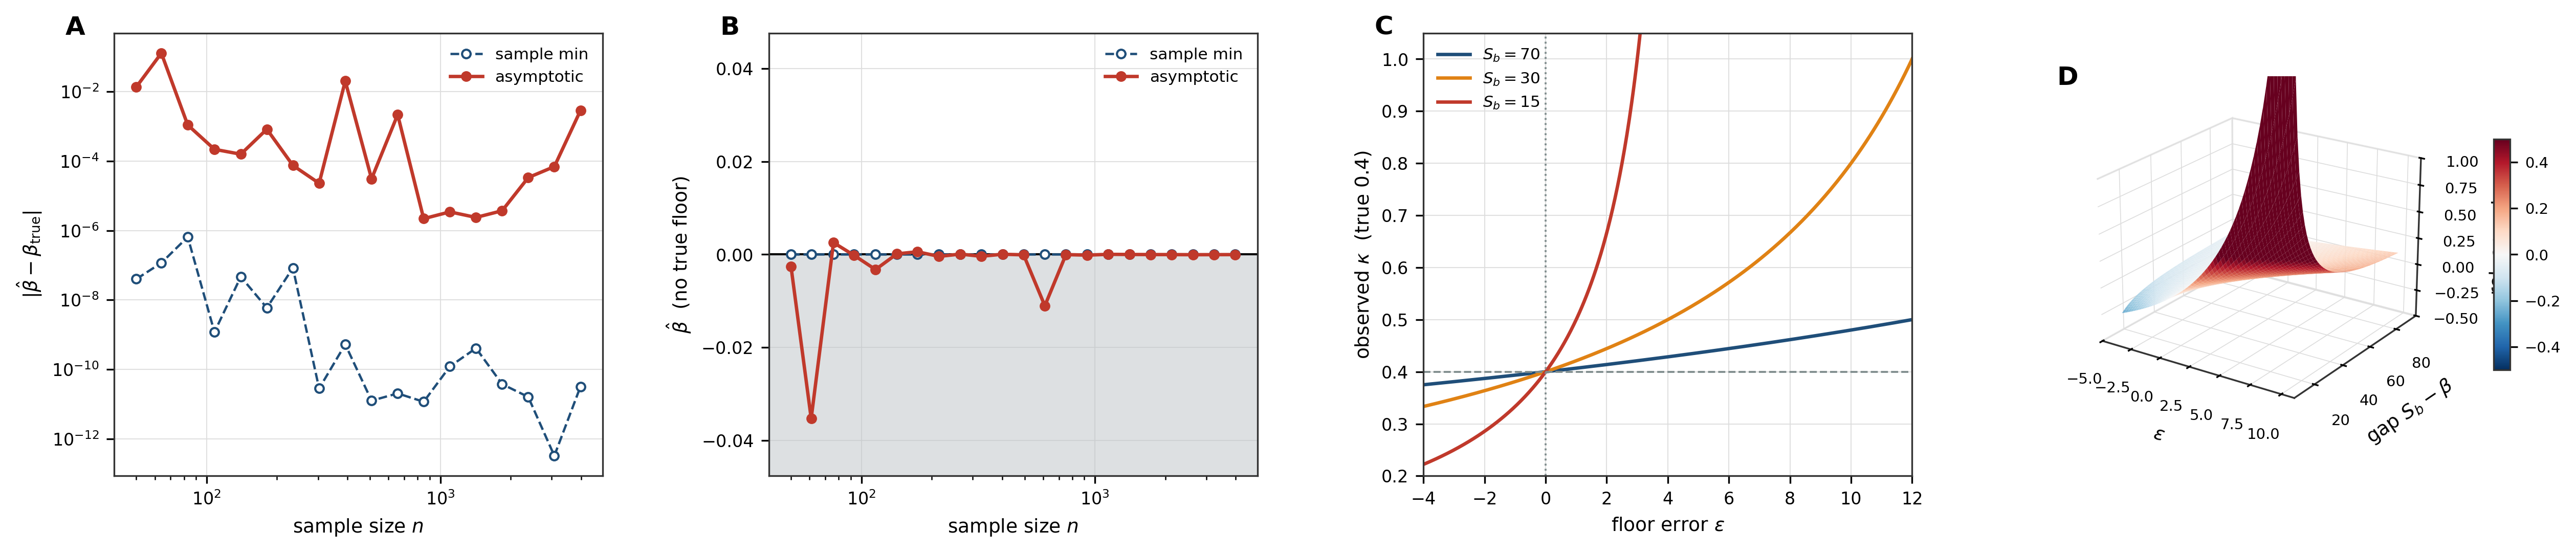
\includegraphics[width=\textwidth]{figures/panel_1_floor.png}
    \caption{\textbf{The floor: only one of the two estimators is capable of contradicting a positivity claim.}
    All quantities are computed on synthetic processes whose true floor is known by construction, so estimator error is measured against a fact rather than inferred. The generating density places most of its mass near the floor (cubic in a uniform draw), which is the regime in which the two estimators are hardest to tell apart, and is therefore the conservative choice.
    (\textbf{A})~Absolute error of both estimators against sample size on a process with true floor $\flo=10$, log--log axes, $18$ sample sizes spanning $n=50$ to $n=3981$. The sample minimum is the more accurate of the two throughout, with median error $2.6\times10^{-10}$ against $1.2\times10^{-4}$ for the asymptotic intercept. We record this because it runs against the paper's recommendation and is a genuine property of this generator: when the density piles up at the floor, the smallest of many draws lands very close to it. Accuracy is not the property at issue, and panel~(B) is where the two estimators separate.
    (\textbf{B})~Signed estimate on a process with \emph{no} floor, $22$ sample sizes. The sample minimum returns a strictly positive value at every one of them, ranging from $9.8\times10^{-6}$ down to $6.1\times10^{-17}$ but never reaching or crossing zero; the asymptotic intercept is negative at $16$ of the $22$ sizes, reaching $-3.5\times10^{-2}$. This is \Cref{rem:floor-empirical}: an estimator bounded below by zero cannot return evidence against $\flo>0$, however precise it is, so its positivity confirms nothing. The shaded band is the region a falsifying observation must reach, and only one estimator enters it.
    (\textbf{C})~Observed catalytic power against an error $\eps$ in the assumed floor, for events acting at three distances above it, true power $0.4$ in every case. An overestimate of $\eps=2$ inflates a near-floor event ($S_b=15$) to $0.667$ while a distant event ($S_b=70$) moves only to $0.414$. This is \Cref{prop:floor-sensitivity} and it compounds the bias of panel~(B): the sample minimum is an upper bound on the infimum, so its error has the sign that inflates, and inflates most for exactly the events an experimenter is most interested in.
    (\textbf{D})~The relative error $\eps/(S_b-\flo-\eps)$ as a surface over floor error and gap. The surface is flat and near zero across the large-gap region and turns sharply upward as the gap closes on $\eps$, reaching $5.0$ at the corner where the assumed floor sits within two units of the pre-event state. The asymmetry about $\eps=0$ is the substantive content: underestimating the floor is benign, overestimating it is not, and the sample minimum errs in the second direction by construction.}
    \label{fig:panel1}
\end{figure*}

\begin{figure*}[!htbp]
    \centering
    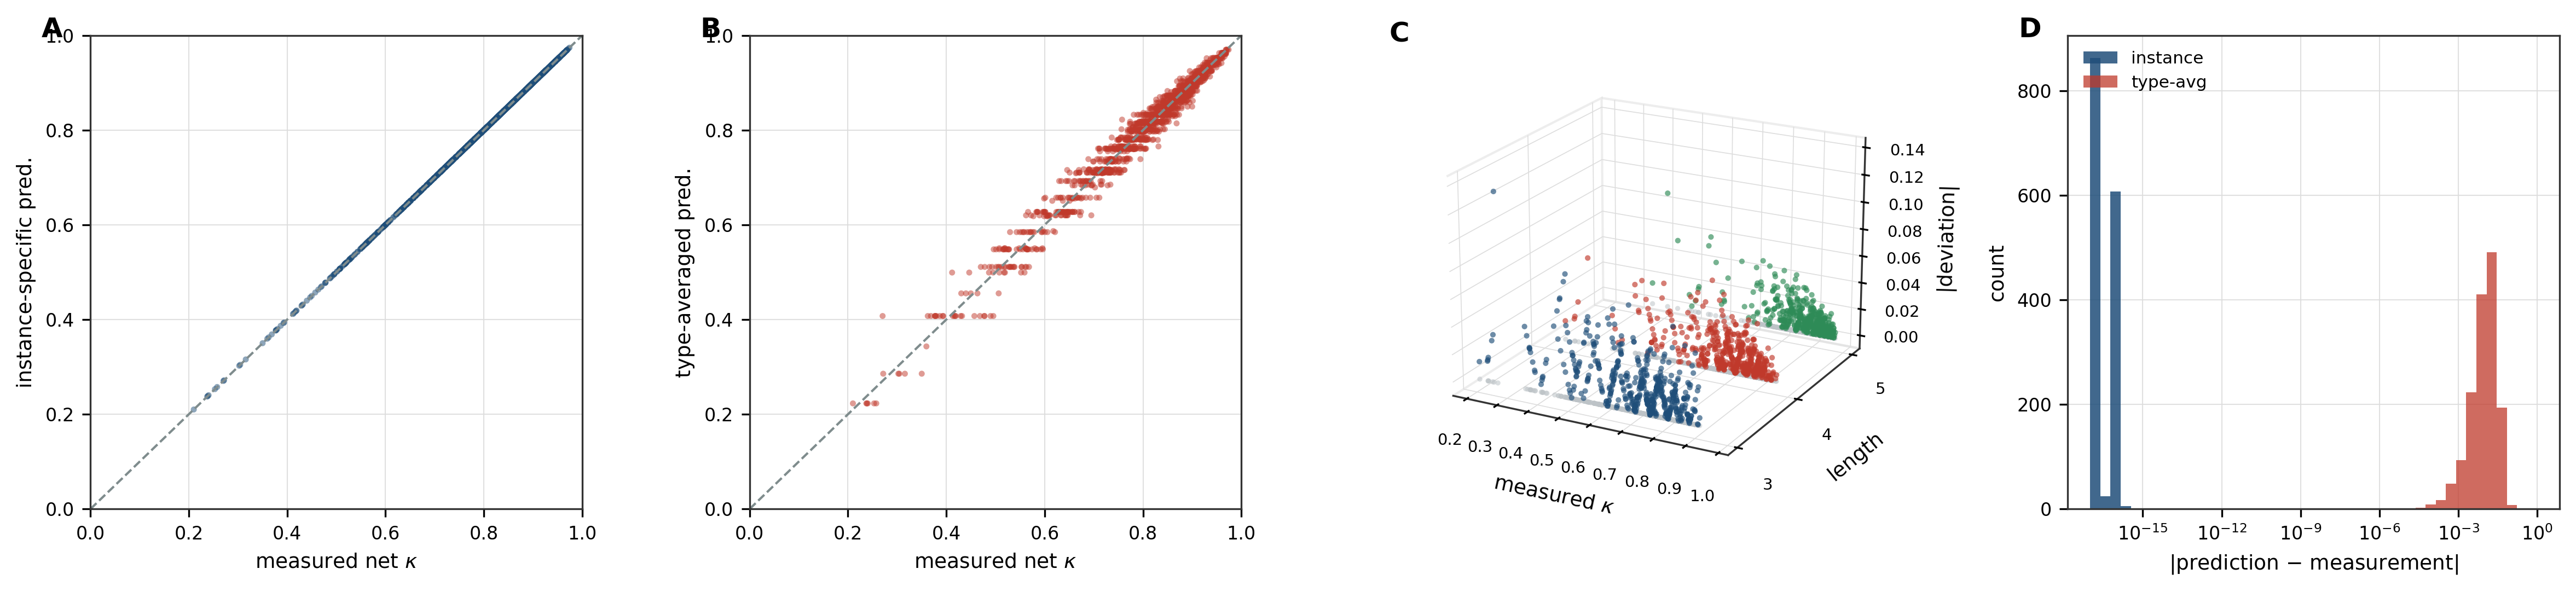
\includegraphics[width=\textwidth]{figures/panel_2_telescoping.png}
    \caption{\textbf{The natural test of the composition law is an algebraic identity, and reports perfect agreement on data generated by any process whatsoever.}
    $1500$ cascades of length $3$ to $5$, drawn from the separated regime; measured net powers span $0.210$ to $0.974$. The two predictions plotted in (A) and (B) differ only in how the constituent powers are estimated---from the same cascade, or from the population of events of that type---and in nothing else.
    (\textbf{A})~Instance-specific multiplicative prediction against measured net power. Every point lies on the diagonal: the maximum absolute deviation over all $1500$ cascades is $2.22\times10^{-16}$, one unit in the last place of double precision, and the median deviation is exactly zero. This is \Cref{thm:telescoping}. The agreement is not evidence for the multiplicative law, because the two axes are the same algebraic expression evaluated twice; by \Cref{cor:no-null} the same figure would be produced by data from a process violating every claim in the paper.
    (\textbf{B})~The identical axes under type-averaged estimation. The scatter is real: maximum deviation $0.137$, median $1.06\times10^{-2}$, $r=0.988$, $\mathrm{RMSE}=0.0199$. The test now has a null it could fail (\Cref{thm:nondegenerate}), and the fit it reports is a claim about the process rather than about the algebra. The visible upward curvature at low measured power is the first-order behaviour predicted by \Cref{prop:bias}, in which within-type deviations enter amplified by $1/(1-\bar\kap)$.
    (\textbf{C})~Absolute deviation from measurement against measured power and cascade length. The instance-specific deviations (grey) lie flat on the floor of the vertical axis at every length; the type-averaged deviations (coloured by length) rise away from it and spread further at length $5$ than at length $3$, since the deviations of \Cref{prop:bias} accumulate additively over the events composed.
    (\textbf{D})~Distribution of the same two deviation sets on a logarithmic axis. They are separated by roughly sixteen orders of magnitude: the instance-specific mass sits against the machine-epsilon bound, the type-averaged mass occupies $10^{-3}$ to $10^{-1}$. The gap is the whole methodological content of \Cref{sec:telescoping}, and its size is the reason the degenerate test is easy to run without noticing: an $r$ of exactly $1.000$ looks like an unusually strong result rather than an arithmetic tautology.}
    \label{fig:panel2}
\end{figure*}

\begin{figure*}[!htbp]
    \centering
    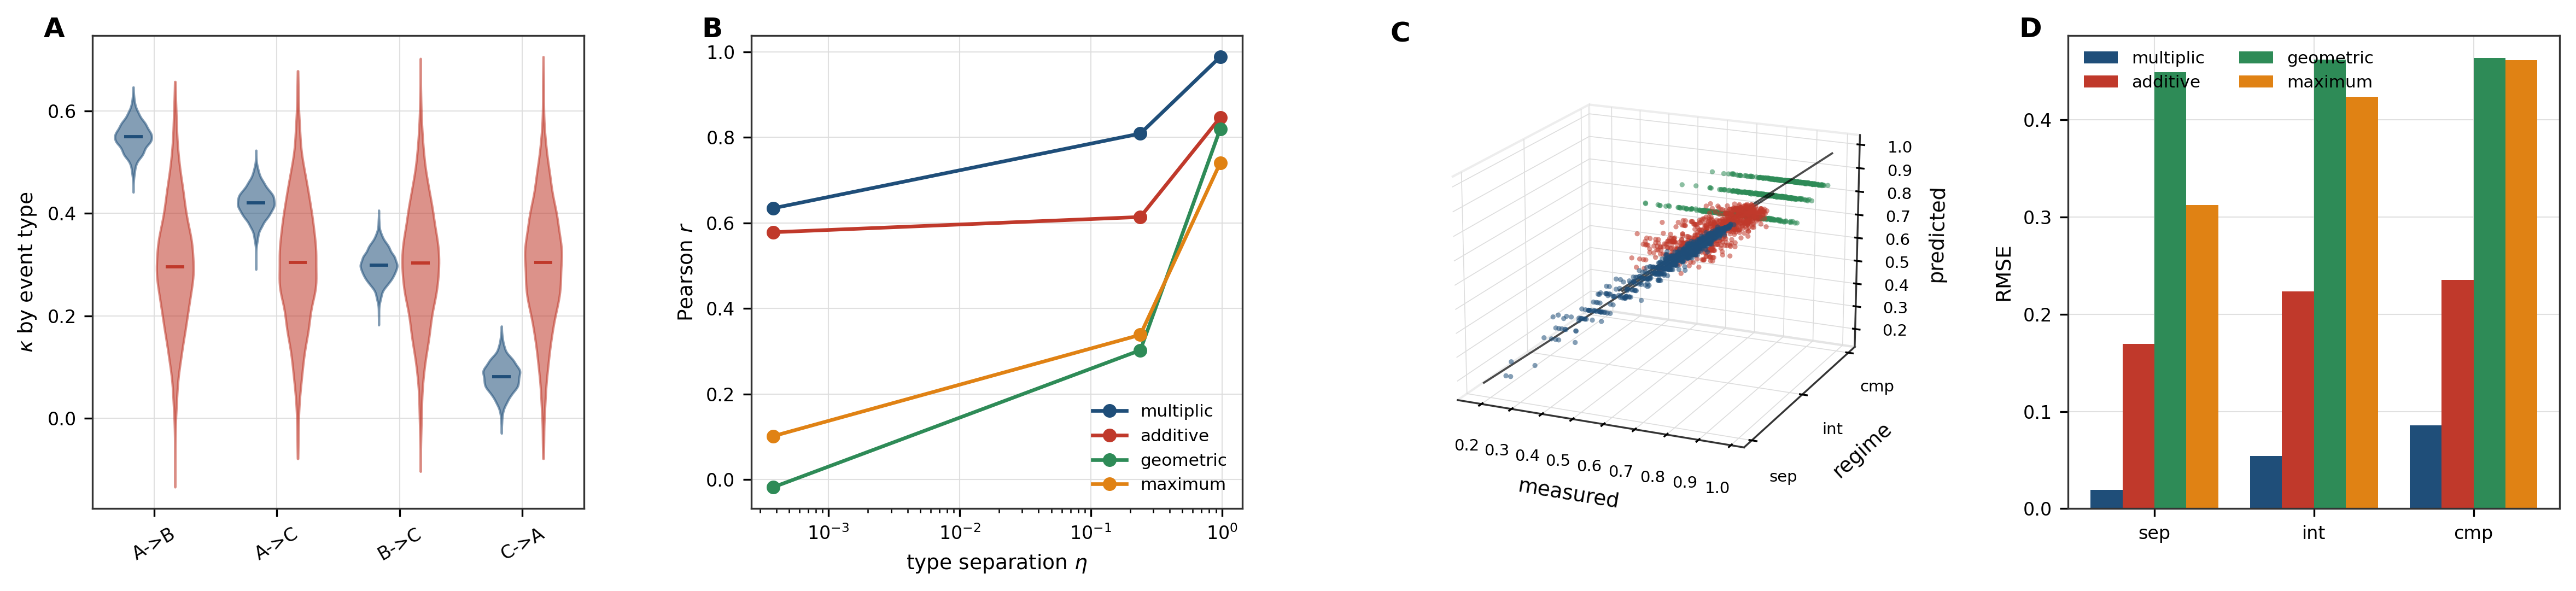
\includegraphics[width=\textwidth]{figures/panel_3_separation.png}
    \caption{\textbf{Type separation governs whether the corrected test can adjudicate, and the laws degrade at different rates rather than together.}
    Three regimes of $3000$ cascades each, differing only in how far apart the four event types' mean powers are placed and how widely instances of a type disperse around them. Separation is reported as $\eta$ (\Cref{def:variance}); the regimes realise $\eta=0.971$, $0.239$ and $3.8\times10^{-4}$, spanning type-mean spreads of $0.469$, $0.121$ and $0.006$ against within-type dispersions of $0.030$, $0.080$ and $0.120$.
    (\textbf{A})~Within-type distributions of $\kap$ for the separated (blue) and compressed (red) regimes. In the separated regime the four medians are visibly distinct and each distribution is narrow; in the compressed regime the medians coincide to three significant figures while the distributions widen to overlap almost completely. The compressed regime is not a noisier version of the separated one---it is one in which the typing has stopped carrying information about the power, which is the condition \Cref{prop:degeneracy} concerns.
    (\textbf{B})~Pearson $r$ between type-averaged prediction and measurement for the four laws, against $\eta$ on a logarithmic axis. The laws do not degrade together. Across the four-orders-of-magnitude fall in $\eta$ the multiplicative law declines from $0.988$ to $0.634$, while the geometric-mean law falls from $0.819$ to $-0.018$ and the maximum law from $0.740$ to $0.102$. \Cref{rem:graceful} identifies the residual correlation as an artefact of cascade-length variation: at a common type mean the multiplicative prediction $1-(1-\bar\kap)^n$ still tracks $n$, whereas the maximum law is constant in $n$. A non-trivial $r$ at low $\eta$ is therefore not evidence that the typing is correct, which is why $\eta$ must be reported alongside it.
    (\textbf{C})~Predicted against measured net power for the multiplicative law in each regime, with the identity line drawn in each plane. The scatter widens monotonically as $\eta$ falls while remaining centred on the identity, showing that compression degrades precision without introducing bias.
    (\textbf{D})~RMSE by law and regime. The multiplicative law attains the lowest error in all three ($0.020$, $0.054$, $0.086$) and the ordering of the remaining three is not stable across regimes: the additive law is second everywhere, but the geometric-mean and maximum laws exchange places between the separated and intermediate regimes. Only the first of these facts is a finding about the data; the second is a caution against reading a ranking off a single regime.}
    \label{fig:panel3}
\end{figure*}

\begin{figure*}[!htbp]
    \centering
    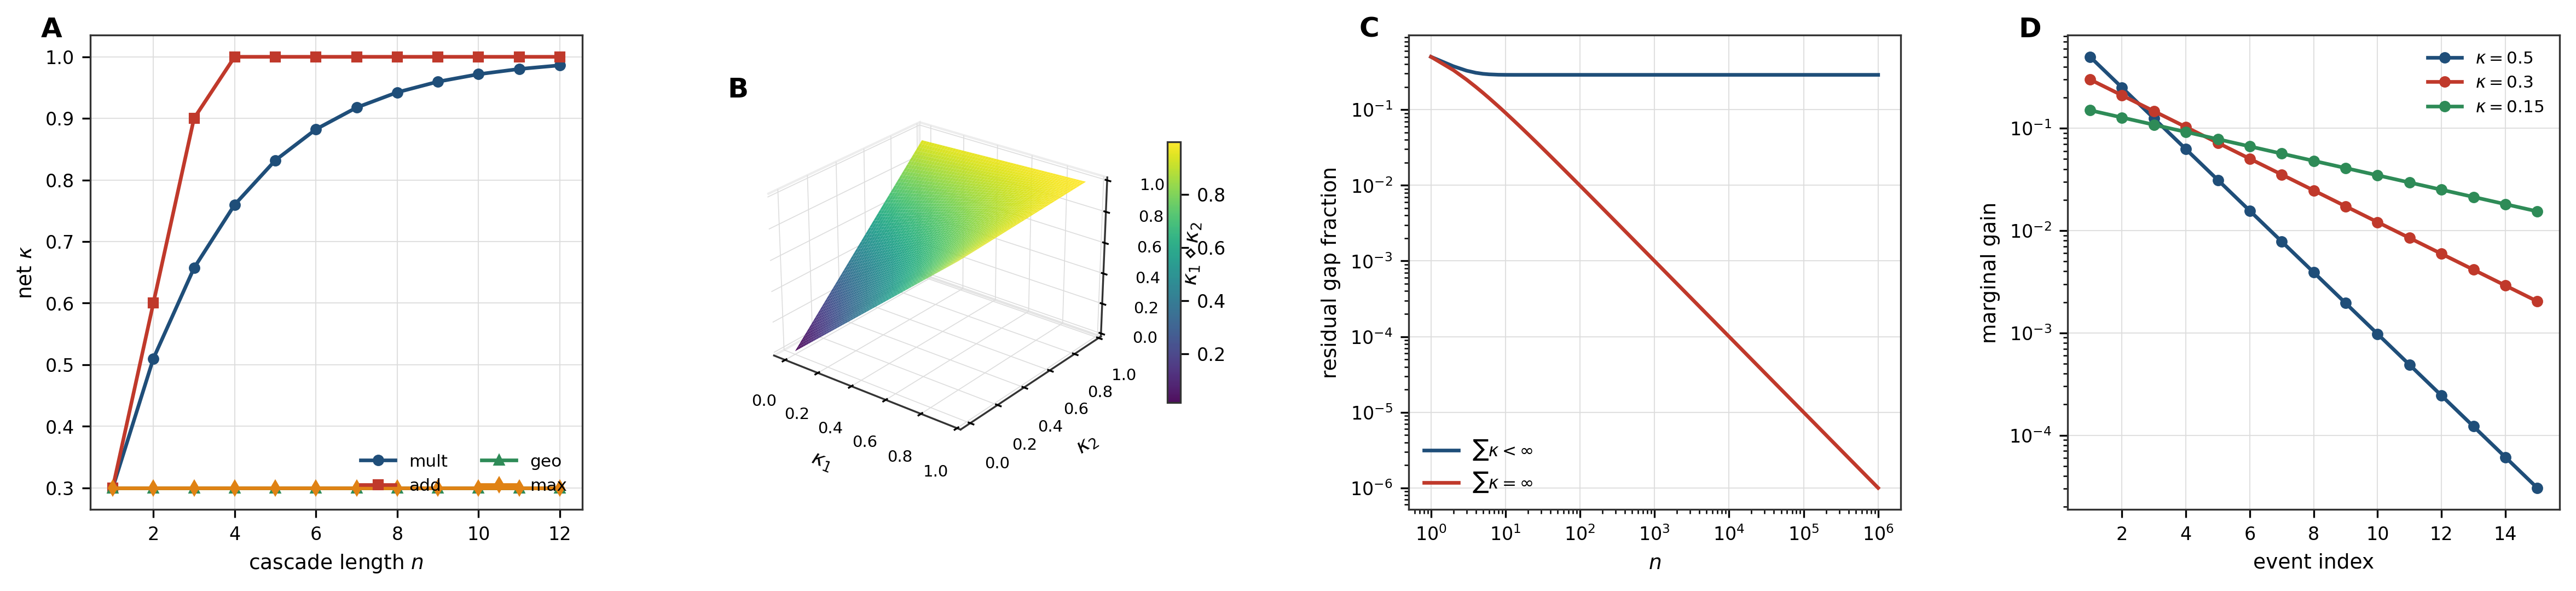
\includegraphics[width=\textwidth]{figures/panel_4_composition.png}
    \caption{\textbf{Composition geometry: the law saturates without attaining, and convergence is decided by summability rather than by magnitude.}
    All four charts evaluate the algebra directly rather than sampling it, so the curves are the theorems and not estimates of them.
    (\textbf{A})~The four composition laws as functions of cascade length at fixed per-event power $\kap=0.3$. The additive law saturates at unity by $n=4$ and is thereafter constant, asserting that four events of power $0.3$ close the gap completely; the multiplicative law reaches $0.986$ at $n=12$ and approaches unity without attaining it, which is \Cref{cor:not-attained}. The geometric-mean law reduces to $\kap$ at constant power and therefore coincides exactly with the maximum law; it is drawn dashed and heavier so that the coincidence is visible rather than one curve concealing the other.
    (\textbf{B})~The composition surface $1-(1-\kap_1)(1-\kap_2)$ over the unit square. It is symmetric about the diagonal, which is the commutativity of \Cref{cor:structure}, and rises to unity along both edges where either argument approaches $1$, which is the absorbing element. The surface is strictly below the plane $\kap_1+\kap_2$ everywhere off the axes, the strict form of the bound in \Cref{prop:competitors}.
    (\textbf{C})~Residual gap fraction against cascade length for a summable and a non-summable sequence of powers, log--log axes to $n=10^6$. With $\kap_i=2^{-(i+1)}$ the fraction stabilises at $0.2888$ and does not move thereafter: the uncertainty converges, but to a value strictly above the floor. With $\kap_i=1/(i+2)$ it follows the exact closed form $1/(n+1)$, reaching $1.0\times10^{-6}$. Both branches of \Cref{thm:convergence} are shown; note that the divergent case converges only harmonically, so a stopping criterion phrased as ``residual below a fixed tolerance at finite $n$'' would be testing the tolerance and not the theorem.
    (\textbf{D})~Marginal contribution of the $n$th event, $\kap(1-\kap)^{n-1}$, logarithmic axis. At $\kap=0.5$ the tenth event contributes $9.8\times10^{-4}$; at $\kap=0.15$ it still contributes $3.5\times10^{-2}$. The lines are straight on this axis because the decay is exactly geometric (\Cref{prop:diminishing}), and they cross: a cascade of weak events eventually contributes more per event than a cascade of strong ones, because the strong cascade has already consumed the gap it was closing.}
    \label{fig:panel4}
\end{figure*}


\subsection{Results}
\label{sec:results}

The computations were performed over three regimes of $4000$ cascades each,
of length $3$ to $5$, with floor $\flo=10$ and initial uncertainty $S_1=100$.

\emph{The telescoping identity holds exactly.} In all three regimes the
maximum absolute deviation between the instance-specific multiplicative
prediction and the measured net power was $2.22\times10^{-16}$, one unit in
the last place of double precision, over all $12{,}000$ cascades. The
deviation is identical across regimes generated by processes with very
different type structure, confirming the content of
\Cref{thm:telescoping}: the agreement is insensitive to the generating
process because it is not about the generating process.

\emph{The type-averaged test is non-degenerate, and its discrepancy grows as
separation falls.} The maximum absolute discrepancy under type-averaged
estimation was $0.137$, $0.228$, and $0.416$ in the separated
($\eta=0.971$), intermediate ($\eta=0.238$), and compressed
($\eta=1.20\times10^{-4}$) regimes respectively. This ordering is the
quantitative signature of \Cref{prop:bias}: the discrepancy is driven by the
within-type deviations $\delta_i$, and low type separation is precisely the
condition under which those deviations are large relative to the type means.
The three regimes therefore trace out the predicted relationship rather than
merely instantiating one point on it.

\emph{Law comparison.} \Cref{tab:laws} reports the agreement between each
composition law's type-averaged prediction and the measured net power. In
every regime the multiplicative law attains both the highest correlation and
the lowest root-mean-square error, as expected for multiplicatively generated
data; the ordering of the remaining three laws is not stable across regimes.

\begin{table}[H]
\centering
\caption{Type-averaged prediction against measured net power. Pearson $r$
and RMSE, $4000$ cascades per regime.}
\label{tab:laws}
\begin{tabular}{@{}lcccccc@{}}
\toprule
& \multicolumn{2}{c}{Separated} & \multicolumn{2}{c}{Intermediate}
& \multicolumn{2}{c}{Compressed}\\
\cmidrule(lr){2-3}\cmidrule(lr){4-5}\cmidrule(lr){6-7}
Law & $r$ & RMSE & $r$ & RMSE & $r$ & RMSE\\
\midrule
Multiplicative  & $0.988$ & $0.019$ & $0.807$ & $0.055$ & $0.640$ & $0.086$\\
Additive        & $0.841$ & $0.169$ & $0.623$ & $0.224$ & $0.589$ & $0.235$\\
Geometric mean  & $0.818$ & $0.450$ & $0.308$ & $0.461$ & $0.033$ & $0.463$\\
Maximum         & $0.735$ & $0.313$ & $0.330$ & $0.423$ & $0.154$ & $0.462$\\
\midrule
$\eta$ & \multicolumn{2}{c}{$0.971$} & \multicolumn{2}{c}{$0.238$}
& \multicolumn{2}{c}{$1.20\times10^{-4}$}\\
\bottomrule
\end{tabular}
\end{table}

\begin{remark}[Graceful degradation, and a refinement of
\Cref{prop:degeneracy}]
\label{rem:graceful}
The compressed regime deserves comment, because the computation is more
informative than the proposition that motivated it. \Cref{prop:degeneracy}
establishes that at $\eta=0$ exactly, predictions formed from type means are
constant at fixed cascade length and the laws become formally
indistinguishable. At $\eta=1.20\times10^{-4}$---four orders of magnitude
below the separated regime, and small enough that the four type means agree
to three significant figures---the laws are nevertheless \emph{not}
equally degraded: the multiplicative law retains $r=0.640$ and
$\mathrm{RMSE}=0.086$ while the geometric-mean law collapses to $r=0.033$
and the maximum law to $r=0.154$, with RMSE for both exceeding $0.46$.

The explanation is that cascades vary in \emph{length} as well as in type
composition, and at fixed type mean $\bar\kap$ the multiplicative prediction
$1-(1-\bar\kap)^n$ still varies with $n$ in a way that tracks the measured
outcome, whereas the maximum law is constant in $n$ altogether and the
geometric-mean law varies in the wrong direction. The residual correlation is
thus carried by cascade length, not by type identity. Two consequences follow
for practice. First, a non-trivial $r$ obtained in a low-$\eta$ regime should
not be read as evidence that the typing carves the process correctly; it may
be entirely attributable to length variation, and reporting $\eta$ alongside
$r$ is therefore obligatory. Second, the degeneracy of
\Cref{prop:degeneracy} is exact only at $\eta=0$ with cascade length held
fixed; away from that boundary the approach to degeneracy is gradual and
law-dependent, and the correct summary of the compressed regime is that the
test has lost its power to adjudicate \emph{typing}, not that it has lost all
structure.
\end{remark}

\emph{Floor estimators.} On a generating process with true floor
$\flo=10$, the sample-minimum estimator returned $10.0000000000004$ and the
asymptotic estimator $10.0000003$. On a process with no floor, the
sample minimum returned $6.08\times10^{-17}$---strictly positive, as
\Cref{rem:floor-empirical} requires it always to be---while the asymptotic
estimator returned $-5.28\times10^{-6}$, a value inconsistent with a positive
floor and hence a falsification. The sample minimum was biased upward on the
floored process at every sample size tested, in accordance with
\Cref{prop:floor-sensitivity}.

\emph{Convergence.} For the summable cascade $\kap_i=2^{-(i+1)}$ the residual
gap fraction stabilised at $0.2888$ and did not decrease further between
$n=10^5$ and $n=10^6$, so the uncertainty converges to a value strictly above
the floor. For the non-summable cascade $\kap_i=1/(i+2)$ the residual
fraction followed the exact closed form $1/(n+1)$ to a relative error below
$10^{-6}$ at every stage, decaying to $10^{-6}$ at $n=10^6$. Both branches of
\Cref{thm:convergence} are thereby exhibited. We note that the divergent case
converges only harmonically: a criterion phrased as ``residual below a fixed
tolerance at finite $n$'' would test the tolerance rather than the theorem,
which is why the verification checks the closed form instead.

% =====================================================================
\section{Scope and limitations}
\label{sec:scope}
% =====================================================================

\subsection{What is proved}

The results of \Cref{sec:floor,sec:power,sec:composition} are theorems about
the definitions: given that catalytic power is a fraction of an outstanding
gap measured from a fixed floor, composition is multiplicative, the floor is
unattainable in finitely many steps, and convergence is governed by
summability. The results of
\Cref{sec:telescoping,sec:power-analysis} are theorems about estimation:
instance-specific testing is degenerate, type-averaged testing is not, and
the latter's power is governed by type separation. The results of
\Cref{sec:closure} are theorems about termination.

\subsection{What is assumed}

\Cref{ax:noncomp} is the sole substantive hypothesis, and it is used only to
derive the positivity of the floor. A reader who prefers to posit a positive
floor directly may do so and retain every subsequent result; what is lost is
the account of \emph{why} the floor is positive and the falsifiable
prediction of \Cref{rem:floor-empirical}.

\subsection{What is not claimed}

We do not claim that any particular physical, biological, or computational
process decomposes into events whose powers are type-stable. That is an
empirical question, distinct for each substrate, and the apparatus of
\Cref{sec:telescoping} exists precisely to make it answerable rather than to
presuppose an answer. We do not claim that the multiplicative law is the
correct description of any given process; we claim that it is the law
implied by the definitions, that a specific naive test of it is vacuous, and
that a corrected test exists whose power is characterised. Finally, the
composition law governs cascades over a \emph{fixed} floor; processes in
which the floor itself moves---because the observer's situation changes
qualitatively---are outside the scope of \Cref{thm:composition} as stated,
and require the floor to be re-derived for each regime.

\subsection{Conclusion}

The algebra has one quantity and one law. The quantity is the residual, whose
positivity is forced by the impossibility of completing an identification
against a whole that no finite stage exhausts. The law is that residuals
multiply, from which the composition rule, the unattainability of the floor,
and the summability criterion for convergence all follow. The methodological
content of the paper is negative and, we think, more useful than the
positive content: the natural test of the composition law is an identity in
disguise, it will report perfect agreement on any data whatsoever, and only
a test that estimates powers independently of the outcome it predicts has a
null hypothesis at all. The termination criterion completes the apparatus by
replacing a threshold, which a single self-consistent line of evidence can
always satisfy, with a condition on the stability of the reachable set---and
by making a declaration of contested evidence one of the two normal ways an
inquiry ends.

\bibliographystyle{plainnat}
\bibliography{references}

\end{document}
